\part{Details}
\label{p:details}

In the second part of these notes, 
we describe the non-trivial response of a beam
detector to gravitational waves, calculate the overlap function
between a pair of detectors, and introduce a promising Bayesian method
to search for the astrophysical background produced by stellar-mass
binary BHs and NSs throughout the universe.

%%%%%%%%%%%%%%%%%%%%%%%%%%%%%%%%%%%%%%%%%%%%%%%%%%%%%%%
\section{Non-trivial detector response}
\label{s:nontrivial_response}

To understand stochastic background searches on a 
more quantitative level, we need to describe the 
non-trivial response of a GW detector to a passing GW.
In Section~\ref{s:optimal_filtering}, we defined the 
overlap function $\Gamma_{12}(f)$
for a pair of detectors, but we didn't specify how 
to calculate it, or how its form differs for different
GW detectors.
In this and the following section, we will develop
the tools that we need to do these calculations.

For simplicity, we will restrict our attention to 
{\em beam detectors}, which use electromagnetic radiation
to monitor the separation of two or more test masses.
Laser interferometers (both ground-based and space-based),
spacecraft Doppler tracking, and pulsar timing arrays
are all examples of beam detectors.
(A resonant-bar detector, like that first used by
Joseph Weber, is a much different type of detector.
Roughly speaking, a resonant bar detector responds
like a giant tuning fork to a passing GW, provided
the GW has frequencies equal to the resonant frequency 
of the bar.)
The response of a beam detector to a passing GW is 
the change in the light-travel time between the two 
masses relative to the nominal light-travel time
This is illustrated schematically in Figure~\ref{f:beam_detectors}.
%
\begin{figure}[htbp!]
\begin{center}
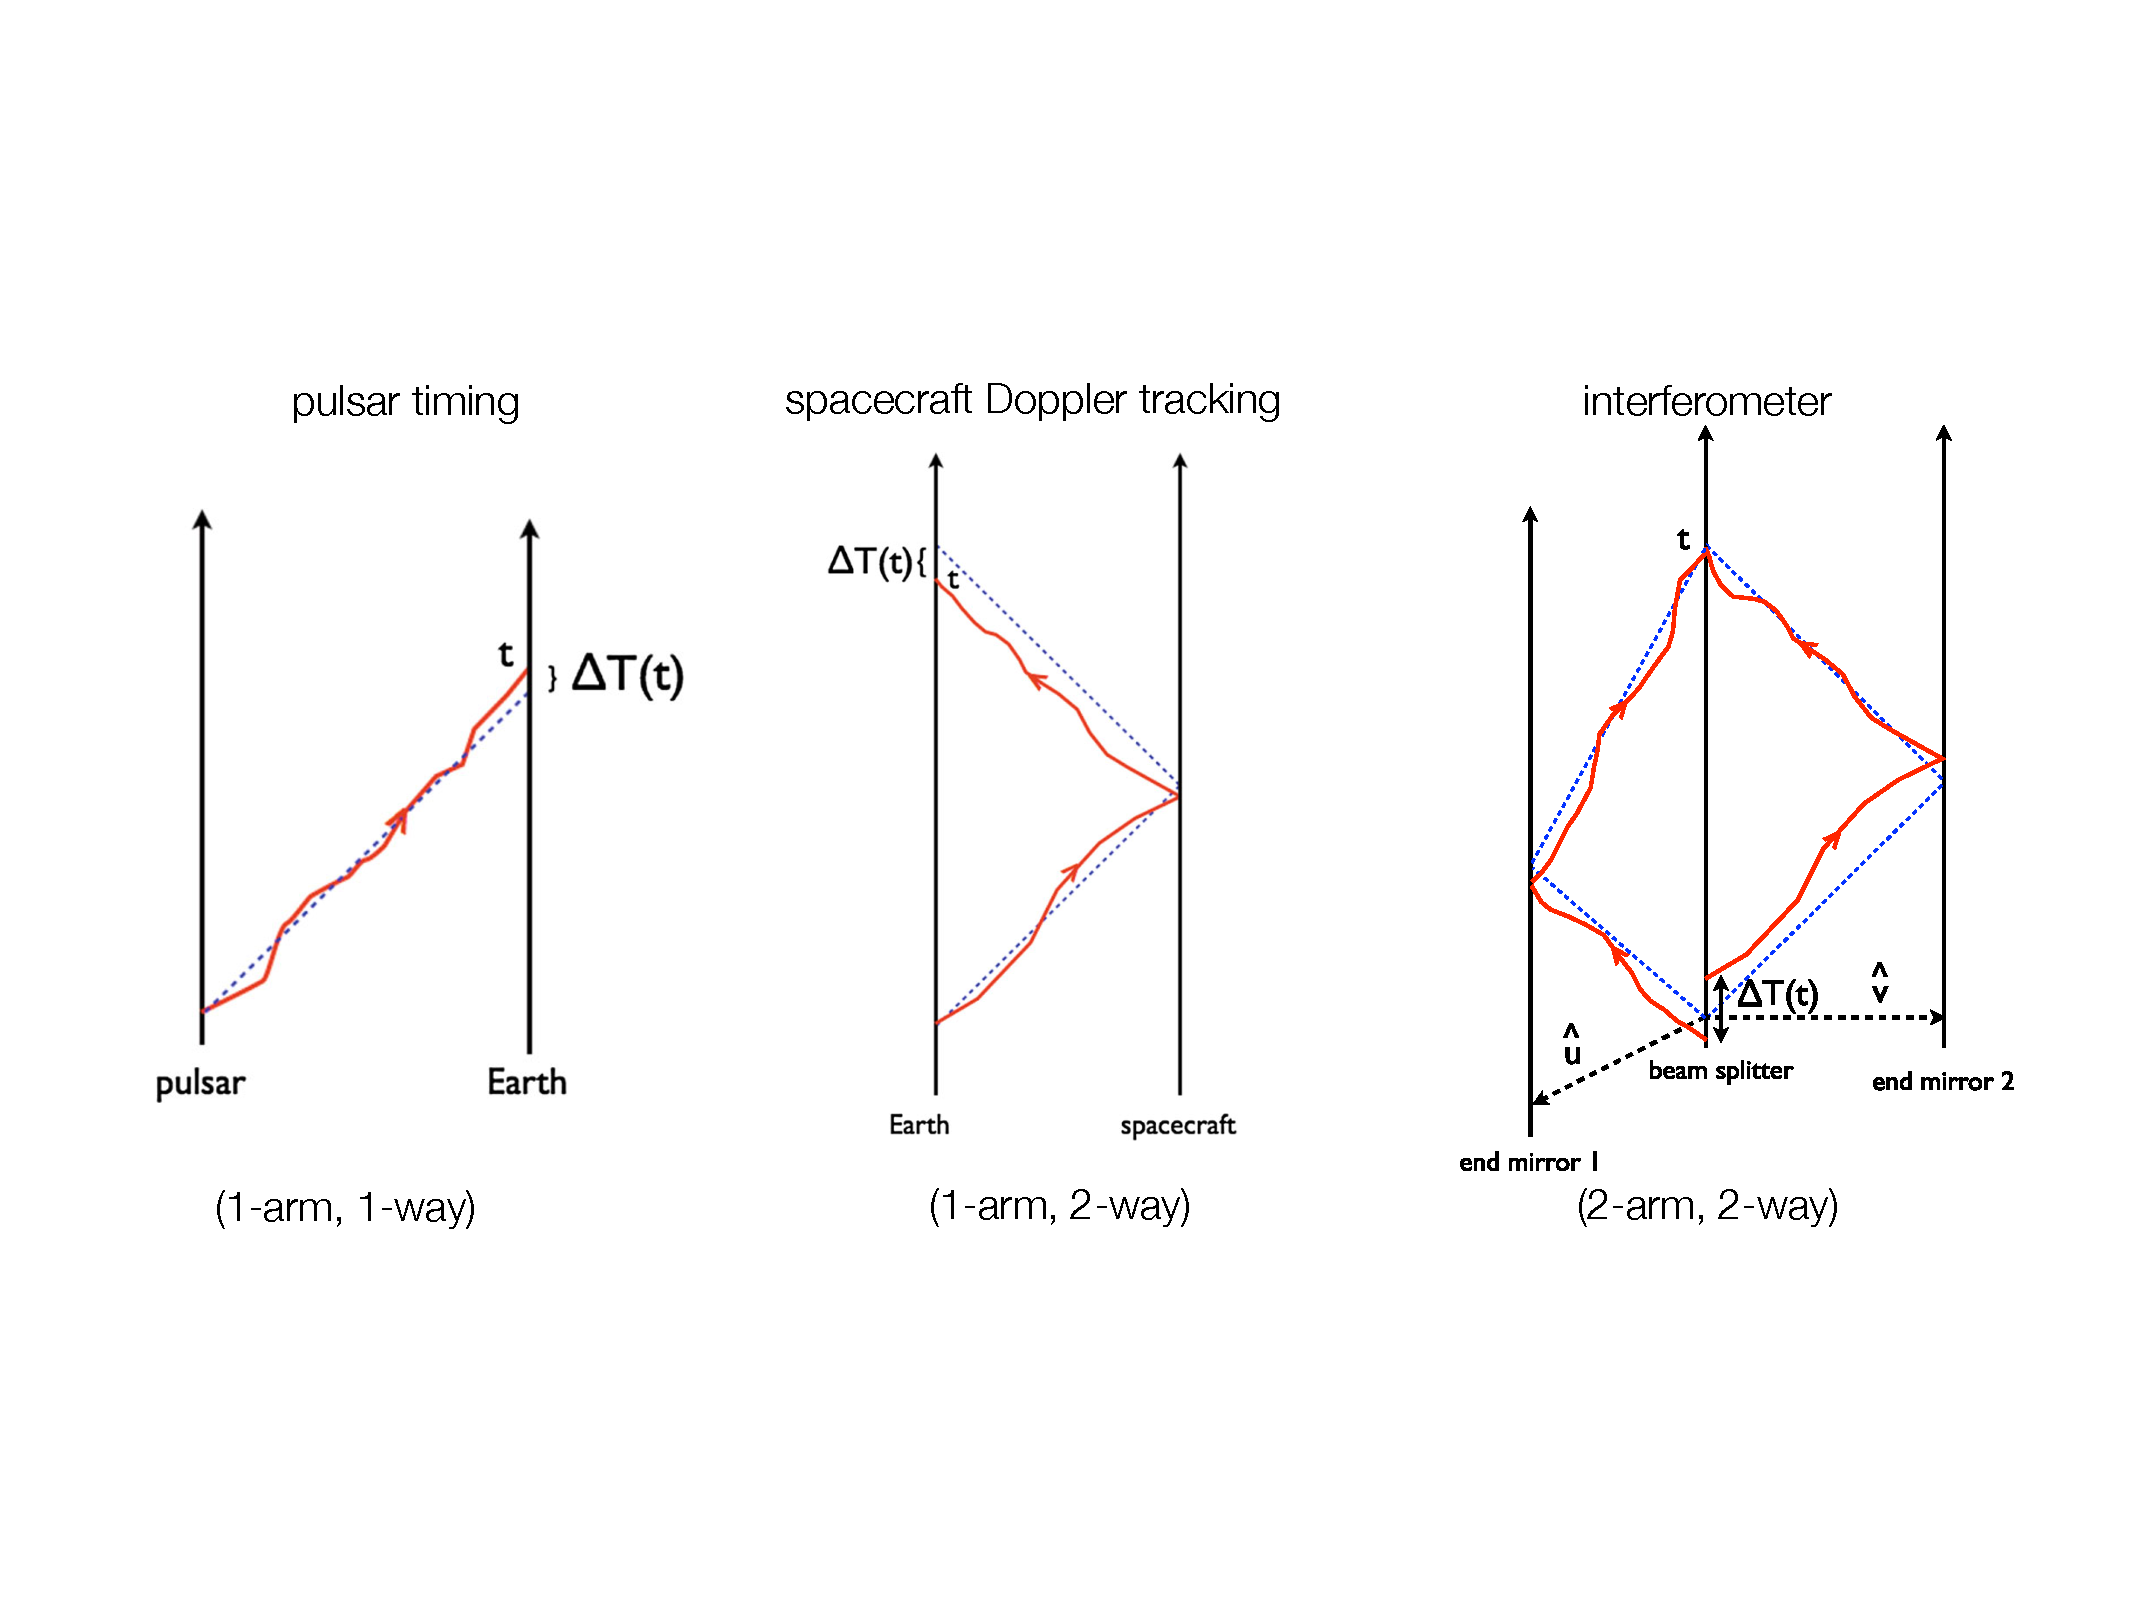
\includegraphics[width=\textwidth]{Figures/beam_detectors}
\caption{Spacetime diagram showing the response of beam
detectors to a passing GW.  
Left column: pulsar timing; middle column: spacecraft Doppler
tracking; right column: interferometer (ground or space-based).
A passing GW perturbs the path of the photon (red trajectory) 
relative to its nominal path in the absence of the wave 
(blue dotted line), leading to a 
difference in the expected arrival time of the photon.
(Figure adapted from \cite{Romano-Cornish:2017}.)}
\label{f:beam_detectors}
\end{center}
\end{figure}
%

In the literature, one might see the detector response
written in terms of strain $\Delta L(t)/L$, 
fractional Doppler frequency $\Delta v(t)/\nu_0$, or 
phase $\Delta\Phi(t)$, instead of the timing residual
$\Delta T(t)$.
Despite the apparent differences in the responses, 
they are all simply related to the timing residual 
response via the relations:
%
\be
\begin{aligned}
&h(t)\equiv \Delta T(t)\quad &({\rm pulsar\ timing})\\
&h(t)\equiv \frac{\Delta L(t)}{L} = \frac{\Delta T(t)}{T}
\quad&({\rm LIGO,\ Virgo,\ }\cdots) \\
&h(t)\equiv \frac{\Delta\nu(t)}{\nu_0}=\frac{\D \Delta T(t)}{\D t}
\quad &({\rm spacecraft Doppler\ tracking})\\
&h(t)\equiv \Delta\Phi(t) = 2\pi \nu_0\,\Delta T(t)
\quad &({\rm LISA})\,.
\end{aligned}
\ee
%
Hence, once we know how to calculate the timing residual
response $\Delta T(t)$, we can easily calculate all the
other quantities listed above.

%%%%%%%%%%%%%%%%%%%%%%%%%%%%%%%%%%%%%%%%%%%%%%%%%%%%%%%
\section{Non-trivial correlations}
\label{s:nontrivial_correlations}

%%%%%%%%%%%%%%%%%%%%%%%%%%%%%%%%%%%%%%%%%%%%%%%%%%%%%%%
\section{What to do in the absence of correlations?}

%%%%%%%%%%%%%%%%%%%%%%%%%%%%%%%%%%%%%%%%%%%%%%%%%%%%%%%
\section{Searching for the background of binary black-hole
mergers}
\label{s:nonstationary}

